\section{Parallel-Series Equivalence}

We consider two networks: a series resistance $R_{S}$ and reactance $X_{S}$, and a parallel resistance $R_P$ and reactance $X_P$, as shown in Fig.\,\ref{Fig:parallelSeriesEquivalent}.
The series and parallel circuits have quality factors $Q_S \equiv X_S / R_S$ and $Q_P \equiv R_P / X_P$ respectively.
The impedance of the series network is \begin{equation}
Z_{S}=R_{S}+iX_{S} , \end{equation}
and the impedance of the parallel network is \begin{equation}
Z_{P}=R_{P}\frac{1}{1+Q_{P}^{2}}+iX_{P}\frac{Q_{P}^{2}}{1+Q_{P}^{2}} . \end{equation}
Setting the series and parallel impedances equal yields \begin{equation}
R_{S}=R_{P}\frac{1}{1+Q_{P}^{2}} \qquad \text{and} \qquad X_{S}=X_{P}\frac{Q_{P}^{2}}{1+Q_{P}^{2}} . \end{equation}
Dividing these equations gives\begin{equation}
Q_S = \frac{X_{S}}{R_{S}}=\frac{X_{P}}{R_{P}}Q_{P}^{2}=Q_{P} . \end{equation}
This is the main result of this section: the quality factors of equivalent parallel and series circuits are equal.

Since the series and parallel quality factors are equal we can drop the subscript and write $Q$ for both of them.
We then rewrite the relations between the series and parallel components as \begin{equation}
R_{P}=R_{S}(1 + Q^2) \qquad X_{P} = X_{S}\frac{1 + Q^{2}}{Q^{2}} \, . \label{eq:sec:parallelSeriesEquivalence:commonQ} \end{equation}
These equations provide a simple way to convert a series circuit to an equivalent parallel one, and vice versa.
For a given series circuit, one computes $Q$ and then uses Eq.\,(\ref{eq:sec:parallelSeriesEquivalence:commonQ}) to compute $X_P$ and $R_P$.
Note that, because the reactances $X_S$ and $X_P$ generally depend on frequency, the value of $Q$ and therefore the equivalence transformation also depend on frequency.


\begin{figure}
\begin{centering}
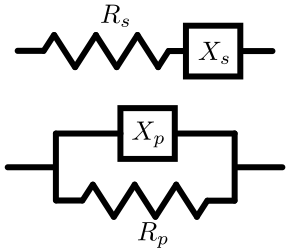
\includegraphics[width=7cm]{parallel_series_equivalent.pdf} 
\par\end{centering}
\caption{Series and parallel circuits. The reactances $X_S$ and $X_P$ can be capacitive or inductive.}
\label{Fig:parallelSeriesEquivalent}
\end{figure}


\subsection{Large $Q$ limit}

In many cases, we have series or parallel circuit fragments for which $Q \gg 1$.
In these cases the transformation equations simplify to \begin{equation}
R_P = Q^2 R_S \qquad X_P = X_S \, . \end{equation}
We explain this intuitively: if the series resistance is low enough that the $Q$ is high, the parallel resistance must be large to ensure it doesn't absorb much energy.
In this case the reactance dominates and is therefore unchanged in the transformation.
